\documentclass[12pt]{article}
\usepackage[english]{babel}
\usepackage[utf8]{inputenc}
\usepackage{fancyhdr}
\usepackage[margin=1in]{geometry}
\usepackage{amsmath}
\usepackage{amsfonts}
\usepackage{amssymb}
\usepackage{scrextend}
\usepackage{enumitem}
\usepackage{tikz}
\usepackage{multirow,array}
\usepackage{float}
\usepackage{graphicx}


\begin{document}

%\vspace*{\stretch{1.0}}
\begin{center}
 	\large\textbf{Methods (draft)}\\
 	\small\textit{Saketh Aleti}
\end{center}
\rule{\textwidth}{1pt}

	
\section{Partial Equilibrium Model}	

The effects of exogenous shocks to crop production and their welfare implications were predicted by applying a set of counterfactual production data to a partial equilibrium model for individual crops. 

First, we used a linear approximation of the supply and demand schedules for each crop $i$ by taking estimates of supply and demand elasticity and computing:
\begin{subequations}
	\begin{align}
	\textbf{Supply: } & Q_{i} = \alpha_{s, i} + \beta_{s, i} P_i 				\\
	\textbf{Demand: } & Q_{i} = \alpha_{d, i} + \beta_{d, i} P_i 	
	\end{align}
\end{subequations}
This was done using current data on the production and prices while assuming the markets were currently in equilibrium. For instance, given the price, quantity, and elasticity of demand of a commodity, we can find:  
\begin{align*}
\beta_{d, i}  &= e_{d, i} \, Q_{i} / P_{i} \\
\alpha_{d, i} &= Q_{i} - \beta_{d, i} P_{i}
\end{align*}

Data on elasticities were obtained from various sources in the literature, while price and quantity data was obtained from FAOSTAT. Counterfactual production values were calculated beforehand with a control quantity and counterfactual quantities for each year; these values modeled relative changes in supply without a demand effect, so they were used to introduce shifts to the supply curves. 
Each shock was introduced to the supply side of the model by adding a coefficient to the supply schedule such that
\begin{subequations}
	\begin{align}
		\textbf{Shocked Supply: } & Q_{i, t}^* = \alpha_{s, i, t}^* + \alpha_{s, i} + \beta_{s, i} P_{i}
	\end{align}
\end{subequations}		
where $Q_{i, t}^*$ is the counterfactual production of crop $i$ in year $t$ and $\alpha_{s, i, t}^*$ is a shift in the supply curve representing the shock; we solve for $\alpha_{s, i, t}^*$ for each crop at each year. Note that the counterfactual data represents relative shocks, so if the counterfactual quantity for year $t$ was $30\%$ smaller than the control, we would have $Q_{i, t}^* = (0.7)Q_i$ where $Q_i$ is present day production. 

After finding the appropriate supply shock, we compute the new equilibrium by solving:
\begin{align*}
Q_{i, t}^* &= \alpha_{s, i, t}^* + \alpha_{s, i} + \beta_{s, i} P_{i, t}^* \\
Q_{i, t}^* &= \alpha_{d, i} + \beta_{d, i} P_{i, t}^* 
\end{align*}
where $P_{i, t}^*$ denotes the price in the counterfactual scenario. From here, we compute the welfare effects of this shock.

\pagebreak

%% Supply and demand graph
\begin{figure}
\centering
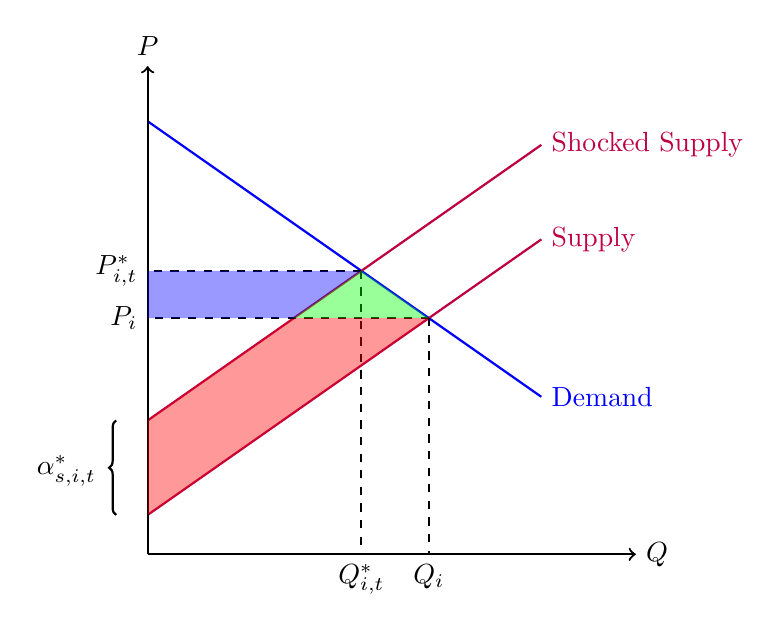
\begin{tikzpicture}[domain=0:5,scale=1,thick]
\usetikzlibrary{calc}                                %allows coordinate calculations.
\usetikzlibrary{decorations.pathreplacing}           %allows drawing curly braces.

% Define linear parameters for supply and demand
\def\dint{5.5}      %Y-intercept for DEMAND.
\def\dslp{-0.7}     %Slope for DEMAND.
\def\sint{0.5}      %Y-intercept for SUPPLY.
\def\sslp{0.7}      %Slope for SUPPLY.
\def\ssh{1.2}       %Y-intercept for SUPPLY2.

\def\tax{1.5}       %Excise (per-unit) tax

% Define Supply and Demand Lines as equations of parameters defined above.
\def\demand{\x,{\dslp*\x+\dint}}
\def\supply{\x,{\sslp*\x+\sint}}
\def\demandtwo{\x,{\dslp*\x+\dint+\dsh}}
\def\supplytwo{\x,{\sslp*\x+\sint+\ssh}}


% Define coordinates.
\coordinate (ints) at ({(\sint-\dint)/(\dslp-\sslp)},{(\sint-\dint)/(\dslp-\sslp)*\sslp+\sint});
\coordinate (intsx) at ({(\sint-\dint)/(\dslp-\sslp)},0);
\coordinate (intsy) at (0,{(\sint-\dint)/(\dslp-\sslp)*\sslp+\sint});

\coordinate (ep) at  (0,{(\sint-\dint)/(\dslp-\sslp)*\sslp+\sint});
\coordinate (eq) at  ({(\sint-\dint)/(\dslp-\sslp)},0);
\coordinate (dint) at (0,{\dint});
\coordinate (sint) at (0,{\sint});


% intercepts of shocked supply
\coordinate (ints2) at ({(\sint+\ssh-\dint)/(\dslp-\sslp)},{(\sint+\ssh-\dint)/(\dslp-\sslp)*\sslp+\sint+\ssh});
\coordinate (ints2y) at (0,{(\sint+\ssh-\dint)/(\dslp-\sslp)*\sslp+\sint+\ssh});
\coordinate (ints2x) at ({(\sint+\ssh-\dint)/(\dslp-\sslp)},0);

% shocked supply quantity at original price
\coordinate (s2p1) at ({((\sint-\dint)/(\dslp-\sslp)*\sslp+\sint)-\sint-\ssh)/\sslp},{(\sint-\dint)/(\dslp-\sslp)*\sslp+\sint});


% DEMAND
\draw[name=demand, thick,color=blue] plot (\demand) node[right] {Demand};

% SUPPLY
\draw[name=supply, thick,color=purple] plot (\supply) node[right] {Supply};

% Shocked Supply
\draw[name=supply2, thick,color=purple] plot (\supplytwo) node[right] {Shocked Supply};

% Draw axes, and dotted equilibrium lines.
\draw[->] (0,0) -- (6.2,0) node[right] {$Q$};
\draw[->] (0,0) -- (0,6.2) node[above] {$P$};
\draw[decorate,decoration={brace},thick]  ($(0,\sint)+(-0.4,0)$) --($(0,\ssh+\sint)+(-0.4,0)$) node[midway,below=-8pt,xshift=-18pt] {$\alpha_{s, i, t}^*$};

\draw[dashed] (ints) -- (intsx) node[below] {$Q_i$};    
\draw[dashed] (ints2) -- (ints2x) node[below] {$Q_{i, t}^*$};                  
\draw[dashed] (ints2) -- (ints2y) node[left] {$P_{i, t}^*$};                       
\draw[dashed] (ints) -- (ep) node[left] {$P_i$};                        

% Fill welfare areas
\fill [fill=blue, opacity=0.4] (intsy) -- (ints2y) -- (ints2) -- (s2p1) -- cycle;
\fill [fill=green, opacity=0.4] (s2p1) -- (ints2) -- (ints) -- cycle;
\fill [fill=red, opacity=0.4] (ints) -- (s2p1) -- ($(0,\ssh+\sint)$) -- ($(0, \sint)$) -- cycle;

\end{tikzpicture}

\end{figure}

Along with computing changes in the consumer and producer surplus, we also compute transfers between the two. In the above figure, the blue region consists of surplus transfered from the consumer to the producer, the red region consists of surplus lost by the producer, and the green region consists of surplus lost by the consumer. 


\end{document}